% \newcommand{\prototitle}{Versuch 2 - Statistik}
% \newcommand{\Fachbereich}{Praktikum Messtechnik}
% \input{../packages/tu_header}

\newcommand{\institut}{Institut f\"ur Telekommunikationssysteme}
\newcommand{\fachgebiet}{Nachrichten\"ubertragung}
\newcommand{\veranstaltung}{Praktikum Nachrichten\"ubertragung}
\newcommand{\pdfautor}{\"Ozg\"u Dogan (326 048), Boris Henckell (325 779)}
\newcommand{\autor}{\"Ozg\"u Dogan (326 048)\\ Boris Henckell (325 779)}
\newcommand{\gruppe}{Gruppe: D03}
%\newcommand{\betreuer}{Betreuer: Mahmoud Felk}


\newcommand{\pdftitle}{Nachrichten\"ubertragung\ Praktikum\ 06}
\newcommand{\prototitle}{Praktikum 06 \\ Digitale \"Ubertragungstechnik: Digitale Empf\"anger}


\input{../../packages/tu_header_8}
 \begin{document}

% \lstlistoflistings
\definecolor{darkgray}{rgb}{0.95,0.95,0.95}
\definecolor{darkolivegreen}{HTML}{01a801}
\definecolor{functionsBlue}{HTML}{32b9b9}
\definecolor{variableRed}{rgb}{1,0,0}
\definecolor{stringBrown}{HTML}{bc8e8e} % f geht nicht

\lstset{
        %\lstset{extendedchars=true} % Umlaute an der richtigen stelle und nicht am Anfang ausgeben
        %basicstyle=\footnotesize\ttfamily,
        basicstyle=\small,
        %
        inputencoding=utf8,
        %
        tabsize=4,
        showspaces=false,
        showtabs=false,
        showstringspaces=true, % no special string spaces
        %
        backgroundcolor=\color{darkgray}, % background
        stringstyle=\color{stringBrown}\fseries, % Strings
        keywordstyle=\color{functionsBlue}\bfseries, % keywords Blau
        identifierstyle=\color{variableRed}, % variablen
        commentstyle=\color{darkolivegreen}, %  comments
        %
        breaklines=true,
        %
        numbers=left,
        numberstyle=\tiny,
        stepnumber=1,
        numbersep=7pt,
        %
        frame=single,
        columns=flexible,
        %
        xleftmargin=-2cm,
        xrightmargin=-1.5cm,
        %
        language=Matlab
}

%---------------------------------------------------------------------
%---------------------------------------------------------------------
%---------------------------------------------------------------------


\section{Einleitung}
\begin{quote}

	In diesem Termin beschäftigen wir uns mit einem Signalangepasstem Empfangsfilter. Wir werden eine zufällige Bitfolge
	mittels eines Formfilters in unterschiedliche Signalformen umwandeln, an der empfängerseite wieder decodieren und
	abschließend die Bitfehlerrate überprüfen. Abschließend werden wir kontrollieren welchen Einfluss die Wahl der
	Sendeform auf die Bitfehlerrate hat.


\end{quote}%beende Einleitung
%--------------------------------------------------------------------
%--------------------------------------------------------------------    

\section{Motivation}
\begin{quote}

	Rauschen kann ein übertragenes Signal beeinflussen und dadurch verfälschen. Bei Binärer Übertragung können daraus
	Bitfehler resultieren, die natürlich unerwünscht sind und vermieden werden sollten. Um daher den Effekt des Rauschens
	und dadurch auch die Bitfehlerrate zu minimieren wird auf der Seite des Empfängers nach der Übertragung
	durch den Kanal ein Signalangepasstes Empfangsfilter verwendet.\\
	Außerdem lässt sich die Bitfehlerrate durch eine geschickte Wahl der Sendeformen weiter minimieren.\\
	Beides werden wir im folgenen umsetzten und durchmessen. 

\end{quote} %section

%--------------------------------------------------------------------
%--------------------------------------------------------------------    


\section{Theorie}
\begin{quote}


    
    
    \end{quote}%section

    Zur Übertragung einer Bitfolge über einen Kanal werden die einzelnen Bits in zu definierenden Sendeformen
    umgewandelt und in dieser Form über den Kanal übertragen. Diese Sendeform kann selbstverständlich während der
    Übertragung durch Rauschen verfälscht werden, was zur folge hat, dass der Empfänger Schwierigkeiten hat zu
    entscheiden, ob das Übertragene Bit ursprünglich eine binäre 1 oder eine  binäre 0 dargestellt hat. Das verwendete
    Sende-Empfangssystem sollte darauf ausgelegt sein, den Empfänger diese Entscheidung so leicht wie möglich zu
    machen.\\
    Als Aussage über die Qualität eines Sende-Empfangssystem dient der ``Signal-To-Noise-Ratio''($SNR$) sowie die
    Bitfehlerrate($P_{Bit}$). Ist nämlich das SNR, sprich das Verhältnis zwischen Sendeleistung zu Rauschleistung, am
    Empfänger möglichst groß fällt es dem Entscheider leichter eine Richtige Entscheidung zu treffen. Die Bitfehlerrate
    sinkt bei großem SNR, da sie die Fehlerrate pro Bit darstellt. Fällt der Entscheider zunehmend richtige
    Entscheidungen sinkt daher die Bitfehlerrate.\\
    Das SNR am Entscheider lässt sich folgendermaßen berechnen:
    
    \begin{equation*}
    	\begin{split}
    		SNR_E = \frac{|f(t_a)|^2}{\sigma_r^2}
    	\end{split}
    \end{equation*}
    
    $|f(t_a)|^2$ stellt in diesem Fall die Amplitude des Nutzsignals zum gegebenen Abtastzeitpunkt und $\sigma_r^2$ die
    Leistung des Rauschens dar.\\
    
    Für die weitere Betrachtung ist es notwendig zwischen Unipolarer und Bipolarer Übertragung zu unterscheiden. Die
    Unipolate Übertragung hat den Vorteil, dass sie mit weniger Aufwand umgesetzt werden kann, da nur eine Sendeform für
    eine der beiden Zustände notwendig ist. Der andere Zustand wird dann durch eine 0 übertragen. Dem entgegen nutzt die
    Bipolare Übertragung für jeden Zustand eine eigene Sendeform. Logischerweise ist diese Implementierung aufwendiger.
    Jedoch zahlt sich dieser Aufwand aus, da der Entscheider SNR für Bipolare Übertragung verbessert.\\
    Um diese Verbesserung mathematisch zu erfassen betrachten wir die Bitenergie($E_b$), die Leistungsdichte von Weißem
    Rauschen($\frac{N_0}{2}$) sowie den Kreuzkorrelationskoeffizenten ($\rho$) ein. Die Bitenergie $E_b$ ist die Energie
    eines Sendeimpulses und errechnet sich mit: \cite{Bitenergie}
    
    \begin{equation*}
    	\begin{split}
    		E_b = \int_{-\infty}^{\infty} \left | s(t)|^2 \right | \mathrm dt
    	\end{split}
        
    \end{equation*}
    
    
    Der Kreuzkorrelationskoeffizient $\rho$ stellt die normierte Kreuzkorrelation zwischen den zwei Sendeimpulsen dar.\cite{kreuz}
    
    \begin{equation*}
    	\begin{split}
    		\rho = \frac{1}{E_b} \int_{0}^{T_{Bit}} s_0(t) \cdot s_1(t) \mathrm dt
    	\end{split}
    \end{equation*}
    
    Abhängig von den Formen der Sendeimpulse kann dieser Koeffizent Werte von $1$, beiden Signalformen stimmen überein,
    bis $-1$, die beiden Signalformen sind genau invertiert zueinander, annehmen.\\
        
    Nun lässt sich mit einigen Umformungen lässt sich die oben aufgeführte Formel für das Entscheider $SNR$ umformen.\\
    Für Unipolare Übertragung ergibt sich dann:
    
    \begin{equation*}
    	\begin{split}
    		max\{SNR_E\} = \frac{2 E_b}{N_0}
    	\end{split}
    \end{equation*}
    
    Im Gegensatz dazu ergibt sich für die Bipolate Übertragung:
    
    \begin{equation*}
    	\begin{split}
    		SNR = \frac{4 E_b}{N_0} (1-\rho)
    	\end{split}
    \end{equation*}
    
    Werden die Sendeformen entgegengesetzt zueinander und mit der selben Bitenergie wie bei der Unipolaren
    Übertragung gewählt steigt das $SNR_{E Bi}$ auf den vierfachen Wert von dem der Unipolaren Übertragung.\\
    
%     In diesem Termin werden wir ausschließlich Bipolare Übertragung mit verschiedenen Sendeformen realisieren und
%     miteinander vergleichen. Bei der selben Bitenergie ver
    
    
    
	
\end{quote}%section Theorie


%--------------------------------------------------------------------
%--------------------------------------------------------------------    
\section{Vorbereitungsaufgabe}
\begin{quote}

    
    Zunächst sollten wir uns als Vorbereitung für den Praktikumstermin mit dem
    Inhalt des Kapitels zu optimalen Empfängerstrukturen aus dem Skript vertraut
    machen und nachvollziehen können.\\
    
    Als nächstes sollte mit Hilfe einer Matlab Datei bipolare Sendeimpulse
    für eine bipolare Übertragung definiert werden. Diese Sendeimpulse sollten als
    Vektoren SF0 und SF1 mit $-1$ und $1$ ein Kreuzkorrelationsergebnis von $\rho
    = 0, -\frac{1}{3}$ oder $-1$ liefern, wobei die Vektoren für $\rho = -1$ und
    $\rho = -\frac{1}{3}$ drei Werte und für $\rho = 0$ vier Werte besitzen
    müssen.\\
    Als Kontrolle dafür, sollte in der Matlab-Datei tatsächlich die
    Kreuzkorrelation durchgeführt und das Ergebnis untersucht werden. Außerdem wird
    die Bitenergie $E_B$ der Sendeimpulse berechnet, wobei die Vektoren als
    zeitkontinuierliche Spannungsverläufe der Dauer $T_B$ angenommen wird, bei
    denen Die Spannungsamplituden nur $+1\ V$ oder $-1\ V$ betragen können.
    Es sollte beachtet werden, dass $T_{SF} = 20\mu s$ konstant bleiben und sich
    somit das $T_B$ mit $T_B = 2 \cdot N \cdot \T_{SF}$ mit N Werten in SF0 bzw.
    SF1 berechnen lässt. Als Bedingung sollte noch gelten, dass die Bitenergien für
    SF0 und SF1 als Paar für ein $\rho$ gleich sein sollten.\\
    
    Als Vorbereitung für den praktischen Teil des Versuchs, sollte eine Funktion
    SAF implementiert werden, welche einen SAF-Empfänger in Matlab realiseren soll.
    Der Input besteht aus DataSamples, ClkSamples und SFSamples, welche gegeben
    sind. der Output dagegen soll dabei der Vektor Values sein, in der die Werte
    nach dem signalangepasstem Filter eingetragen sein sollen.\\
    \TODO{Boris: kannst du hier noch genauer erklären wie die Funktion funzt?}
    
    
    Nach der Implementierung der SAF-Funktion sollten wir uns mit dem
    Versuchsaufbau und der Durchführung vertraut machen und  ein Blockschaltbild
    dazu entwerfen. Die genaue Vorgehensweise ist in dem Abschnitt Durchführung
    detaliert erläutert. Hier ist das entworfene Blockschaltbild zu dem Versuch:\\
    
    \begin{figure}[H]
        \centering
            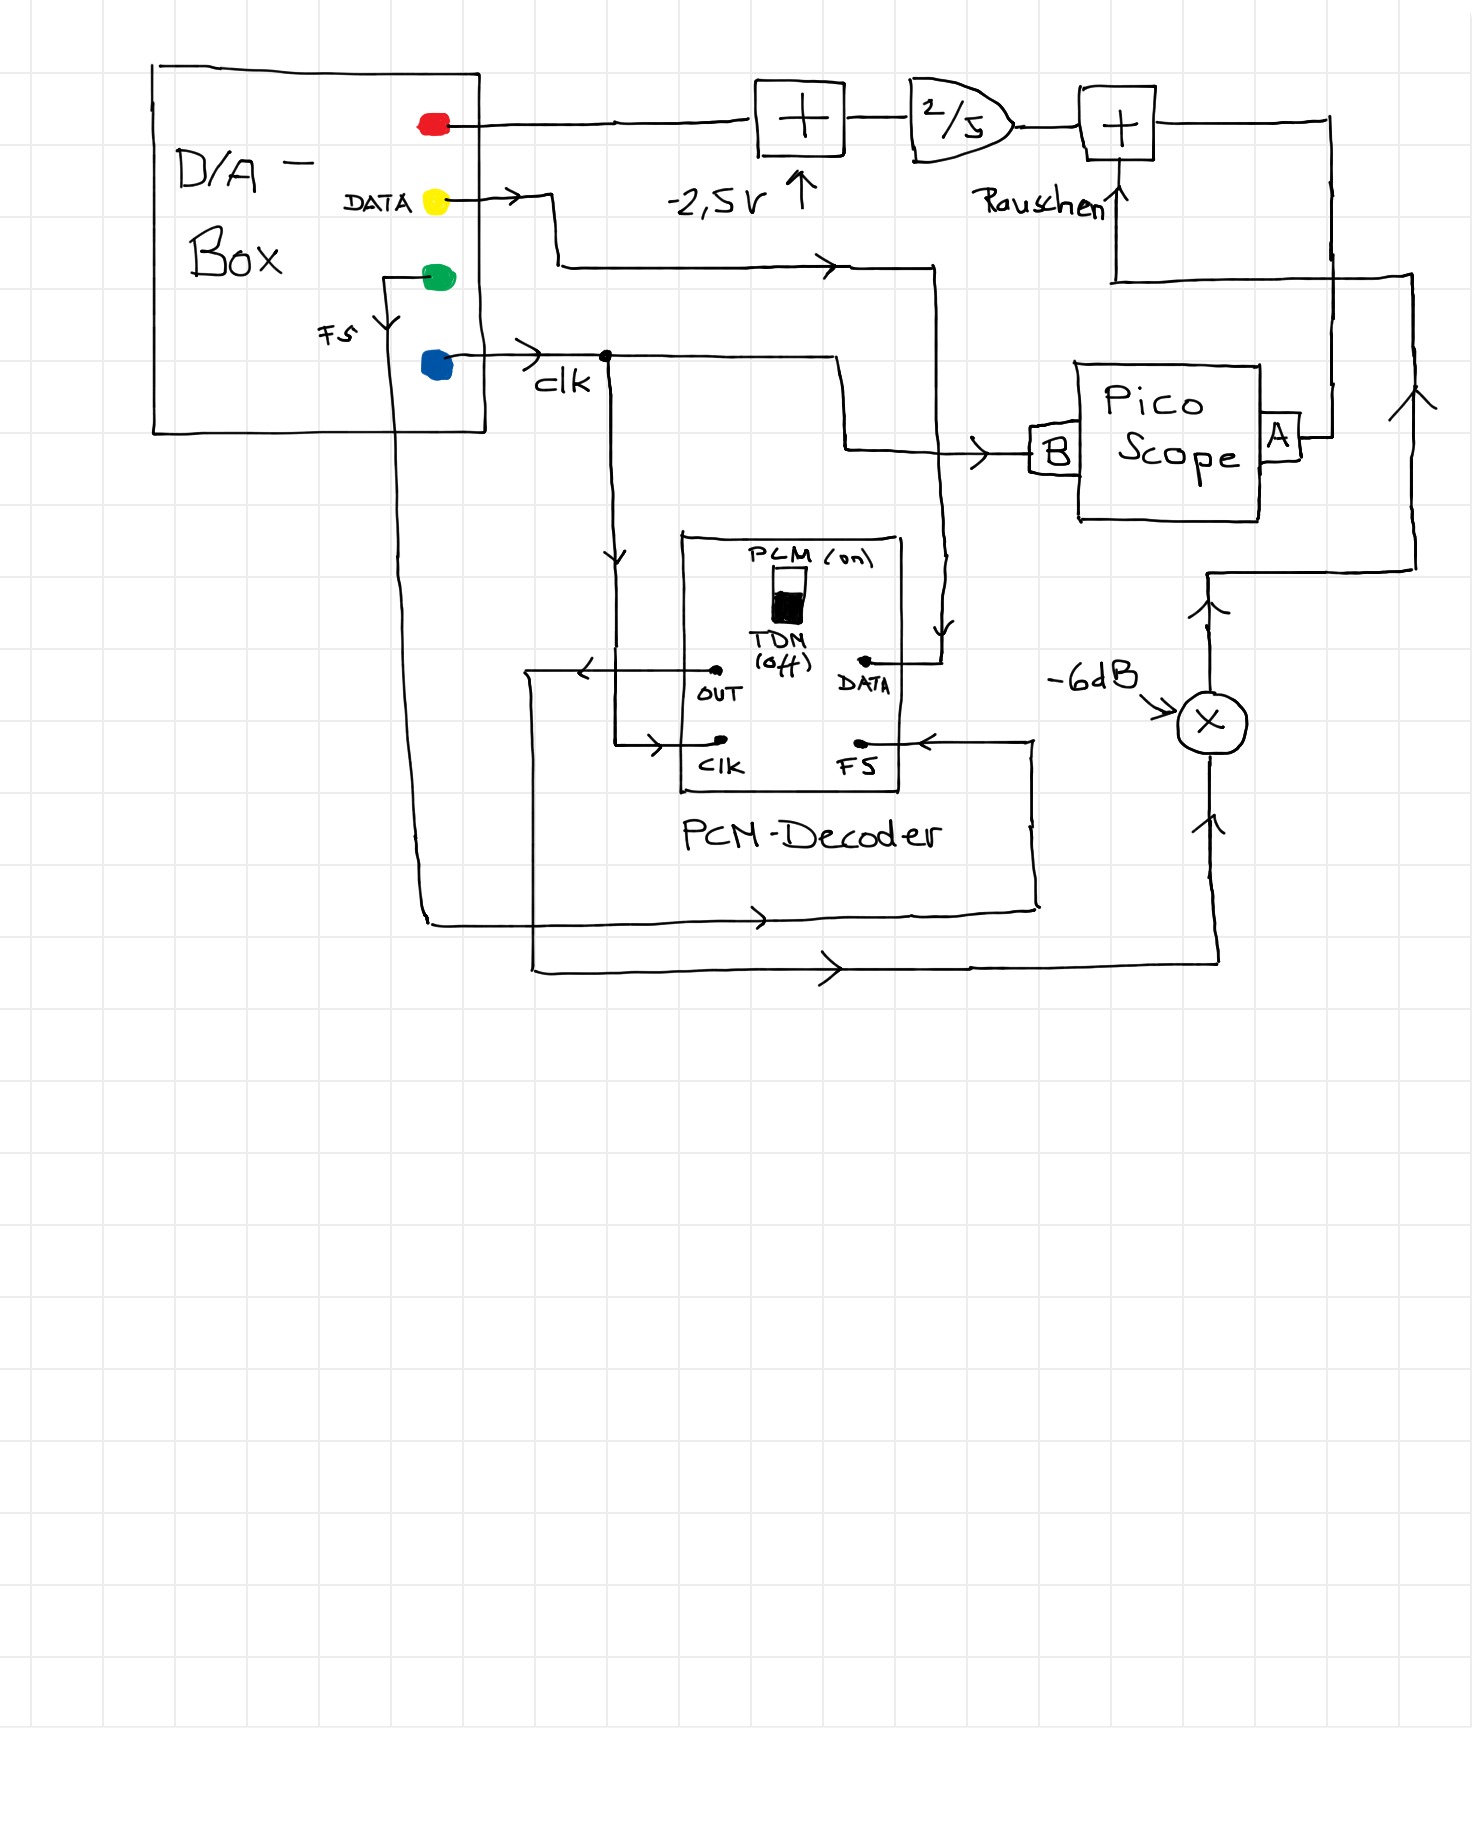
\includegraphics[scale=0.45, trim = 1.5cm 15cm 1cm 0cm,
            clip]{./Bilder/Blockschaltbild.png}
                \caption{Blockschaltbild des Versuchsaufbau}
        \end{figure}
        
    
    Um die implementierte Funktion SAF zu überprüfen, führten wir mithilfe der
    vorgegebenen ENue\_SAF\_Messumgebung.m durch, welche das Hauptprogramm der
    Messung darstellt. Mit dem Parameter Simulation (für die Vorbereitung
    bleibt dieser bei $1$) kann man entscheiden, ob die Ausgabe und
    Einstellungen des Steckbretts simuliert werden, oder ob die Daten über die 
    D/A-Box ausgegeben und per PicoScope eingelesen werden. Mit dem Parameter
    SAF kann man einstellen, ob mit dem DataSignal eine Sendeformung und dem
    Empfangssignal eine signalangepasste Filterung durchgeführt wird. Weiterhin
    sollten wir für die Vorbereitung die Kanal- und Filtereinstellungen nicht
    verändern, wohingegen der NoiseFaktor, welcher den Faktor des Rauschens
    einstellt, variiert werden durfte um die Leistung AWGN (additive white
    Gaussain noise) des Kanals zu beeinflussen.\\
    Mit der Funktion Channel führt man die Übertragung entweder als
    Simulation oder auf dem ETT aus, wobei die Einstellungen der Simulation
    denen des wirklichen Aufbaus entsprechen. Es wird ein Rückgabevektor Y
    ausgegeben, welcher die Werte nach der Abtastung des Kanals enthält.
    Wenn SAF deaktiviert ist, wird eine einfache Nachabtastung mit einem
    Schwellwert von $0V$ durchgeführt.\\
    Außerdem entspricht der Rückgabewert Noise einer Rauschmessung des Kanals,
    wozu eine 0-Bit-Folge gesendet und das Empfangssignal ohne SAF oder
    Nachabtastung als PuciScope-Sample-Signal zurückgegeben wird. Dieses Signal
    enthält ungefähr $10000$ Samples.\\
    
    
    Zuletzt sollte beantwortet werden, wie der Multiplikationsfaktor für das
    Rauschen variiert werden müsste, damit die Wasserfallkurve ausreichend ermittelt werden kann.
    Im Versuch beträgt das Rauschen dabei $-6 dB$.
    
    \end{quote}%Theorie
    % beenden

	
	Zunächst sollten wir uns als Vorbereitung für den Praktikumstermin mit dem
	Inhalt des Kapitels zu optimalen Empfängerstrukturen aus dem Skript vertraut
	machen und nachvollziehen können.\\
	
	Als nächstes sollte mit Hilfe einer Matlab Datei bipolare Sendeimpulse
	für eine bipolare Übertragung definiert werden. Diese Sendeimpulse sollten als
	Vektoren SF0 und SF1 mit $-1$ und $1$ ein Kreuzkorrelationsergebnis von $\rho
	= 0, -\frac{1}{3}$ oder $-1$ liefern, wobei die Vektoren für $\rho = -1$ und
	$\rho = -\frac{1}{3}$ drei Werte und für $\rho = 0$ vier Werte besitzen
	müssen.\\
	Als Kontrolle dafür, sollte in der Matlab-Datei tatsächlich die
	Kreuzkorrelation durchgeführt und das Ergebnis untersucht werden. Außerdem wird
	die Bitenergie $E_B$ der Sendeimpulse berechnet, wobei die Vektoren als
	zeitkontinuierliche Spannungsverläufe der Dauer $T_B$ angenommen wird, bei
	denen Die Spannungsamplituden nur $+1\ V$ oder $-1\ V$ betragen können.
	Es sollte beachtet werden, dass $T_{SF} = 20\mu s$ konstant bleiben und sich
	somit das $T_B$ mit $T_B = 2 \cdot N \cdot \T_{SF}$ mit N Werten in SF0 bzw.
	SF1 berechnen lässt. Als Bedingung sollte noch gelten, dass die Bitenergien für
	SF0 und SF1 als Paar für ein $\rho$ gleich sein sollten.\\
	
	Als Vorbereitung für den praktischen Teil des Versuchs, sollte eine Funktion
	SAF implementiert werden, welche einen SAF-Empfänger in Matlab realiseren soll.
	Der Input besteht aus DataSamples, ClkSamples und SFSamples, welche gegeben
	sind. der Output dagegen soll dabei der Vektor Values sein, in der die Werte
	nach dem signalangepasstem Filter eingetragen sein sollen.\\
	\TODO{hier noch genauer erklären wie die Funktion funzt}
	
	
	Nach der Implementierung der SAF-Funktion sollten wir uns mit dem
	Versuchsaufbau und der Durchführung vertraut machen und  ein Blockschaltbild
	dazu entwerfen. Die genaue Vorgehensweise ist in dem Abschnitt Durchführung
	detaliert erläutert. Hier ist das entworfene Blockschaltbild zu dem Versuch:\\
	
	\TODO{Blockschaltbild zeichnen und einfügen}
	
	
	
	
	\end{quote}%Theorie
	% beenden

%--------------------------------------------------------------------
%--------------------------------------------------------------------    

    
\section{Labordurchführung}
\begin{quote}
    
    \subsection{Aufgabe 2.1 - Aufbau des Versuches}
    \begin{quote}
        
        Die erste Aufgabe des Praktikums beschäftigt sich fast ausschließlich
        mit dem Aufbar des Versuches, um den Signalverlauf mit der Matlab
        Funktion\\ 
        ParallelOUT($[0 1 0 1 0 1 0],100$) zu untersuchen. Dazu wird
        die D/A-Box, welcher an den Computer angeschlossen und somit über
        die Matlab Dateien steuerbar ist, als Quelle für jegliche verwendete
        Signale verwendet. Die D/A-Box besitzt vier Ausgänge, die mit
        unterschiedlichen Farben gekennzeichnet sind. Der rote Ausgang gibt das
        DataSignal aus. Dieser kann eine Amplitude von $0V$ oder $5V$ besitzen.
        Um ihn auf den von uns erwünschte Spannungsbereich von $\pm 1V$ zu
        bringen, wird dieses Signal zunächst mit einer Gleichspannung von
        $-2.5V$ aus der variablen Spannungsquelle des Steckbretts addiert und
        danach mit einem Faktor von $\frac{2}{5}$ gedämpft. Damit erreichen wir
        den nötigen Spannungsbereich, welcher auf dem A Kanal des PicoScopes
        kontrolliert wird.\\
        Der blaue Ausgang der D/A-Box gibt das Clock-Signal wieder. Dieser wird
        auf den B Kanal des PicoScope geführt und ebenfalls kontrolliert.\\
        Als nächstes wird der PCM Decoder mit der D/A-Box verbunden, indem das
        Clock-Signal auch auf den Clock-Eingang des Decoder geführt wird.
        Weiterhin wird das Signal aus dem grünen Ausgang der Box, welcher das
        Frame-Signal (FS) wiedergibt, mit dem FS-Eingang des Decoders
        und die PCM-codierten Datenworte, die aus dem gelben Ausgang der Box
        entnommen werden können, mit dem PCM Data-Eingang des Decoders
        kontaktiert. Wichtig ist auch, dass der Schalter auf dem Decoder Modul
        auf PCM geschaltet ist und nicht auf TDM.\\
        Somit ist der PCM Decoder mit allen Signalen beliefert, die er zum
        decodieren braucht. Daher kann man nun das Output Signal verwenden,
        welcher eine Spannung des Faktors wiedergibt, die für die
        Verstärkung oder Dämpfung des Rauschens dient. Diese Spannung wird an
        einem Multiplikator mit dem $-6 dB$ Rauschen multipliziert und an dem
        Addierer mit Multiplikatoren mit dem DataSignal, welcher bereits auf den korrekten Spannungsbereich
        eingestellt wurde, addiert. Das Ergebniss dieser Addition wird weiterhin
        auf den A Kanal des PicosScopes geführt und ausgewertet.\\
        
        Zuletzt wird das verrauschte Signal überprüft, indem mit der Funktion
        PCM\_Decod(192) ein Verstärkungsfaktor für das Rauschen gesetzt wird.
        Das verrauschte Signal wird mithilfe der PicoScope-Software und der
        Matlab-Funktion ParallelOUT($[0 1 0 1 0 1 0],100$) dargestellt und auch
        mit den Werten $0$, $128$ und $255$ untersucht.
        
        \TODO{Foto vom Aufbau einfügen}
        
    \end{quote}%Ende Durchführung 1
    
    \subsection{Aufgabe 2.2 - Bitfehlermessung}
    \begin{quote}
    
        Das Ergebnis der Bitfehlermessung sollte die Darstellung von
        unterschiedlichen Wassefallkurven sein. Dafür wurden am Ende die
        Wasserfallkurven für die drei unterschiedlichen $\roh$ untersucht,
        welche wir bereits in der Vorbereitung untersucht hatten. Es wurden die
        BER-Messungen aller drei $\roh$-Werte mit $15$ verschiedenen, sinnvollen
        Verstärkungsfaktoren für das Rauschen durchgeführt. Dabei sollten wir
        beachten, dass für größere SNR-Werte die Steigung stärker und eine BER
        von $0$ für ein vorhandenes Rauschen nicht aussagekräftig ist, wenn die
        Messung des BER eine minimale Auflösung von $10^-4$ besitzt. Danach
        wurden die Bitfehlerraten der übertragenen Informationsbits für
        den optimalen Abtastzeitpunkt $T_B$ gemessen und in ein Diagramm
        zusammengefasst. Dieses Diagramm enthält nun die Wasserfallkurven von
        $\roh = -1$, von $\roh = -\frac{1}{3}$ und von $\roh = 0$ mit $15$
        Messwerten.\\
        Die Ergebnisse wurden geplottet und in der Auswertung diskutiert.  
          
    \end{quote}%Ende Durchführung 2

\end{quote}%beende Labordurchführung

%--------------------------------------------------------------------
%--------------------------------------------------------------------    

    
\section{Auswertung}
\begin{quote}
    
    \subsection{Vorbereitungsaufgabe}
    \begin{quote}
        
    \end{quote}  % Ende Subsection Vorbereitungsaufgabe
    
    \subsection{Aufgabe 2.1 - Aufbau des Versuches}
    \begin{quote}
        
        Da diese Aufgabe nur zum korrekten Aufbau des versuchs gedient hat, gibt
        es hier keine Ergebnisse zu diskutieren.
        
    \end{quote}  % Ende Auswertung Aufbau des Versuches
    
    \subsection{Aufgabe 2.2 - Bitfehlermessung}
    \begin{quote}
        \TODO{Aufgabe 2.2} \\
    \end{quote}  % Ende Auswertung Bitfehlermessung
            
\end{quote}%beende Auswertung

%--------------------------------------------------------------------
%-------------------------------------------------------------------- 
    
\section{Zusammenfassung}
\begin{quote}

    \TODO{Zusammenfassug schreiben} \\
\end{quote}%beende Zusammenfassung
         

%--------------------------------------------------------------------
%--------------------------------------------------------------------    


\begin{thebibliography}{999}
      \bibitem {Bitenergie} Prof. Dr.-Ing. Sikora, Thomas; Prof. Dr.-Ing. Noll, Peter: Einführung in die
      Nachrichtenübertragung, S.356
      \bibitem {kreuz} Prof. Dr.-Ing. Sikora, Thomas; Prof. Dr.-Ing. Noll, Peter: Einführung in die
      Nachrichtenübertragung, S.363
%     \bibitem {PCM_Decodierung} Prof. Dr.-Ing. Sikora, Thomas; Prof. Dr.-Ing. Noll, Peter: Einführung in die
%      Nachrichtenübertragung, S.276
%      



%Name, Vorname.; evtl. Name2, Vorname2.: Titel des Dokumentes
%oder Buches, Zeitschrift/Verlag/URL (Auflage, Erscheinungsort, -jahr), ggf. Seitenzahlen
% \bibitem {PasevalscheTheorem} \url{https://de.wikipedia.org/wiki/Parsevalsches_Theorem}, Zugriff
% 23.05.2012
\end{thebibliography}

\end{document}
        
